\section{External Interface Requirements}

\subsection{User Interface}
The following mock ups represent a basic idea of how the Mobile Application
and the Web Interface are supposed to look like.
Through the smart-phone application and web interface, users have access to complete SafeStreets functionalities, including the possibility of notifying violations.

\begin{figure}
  \centering
  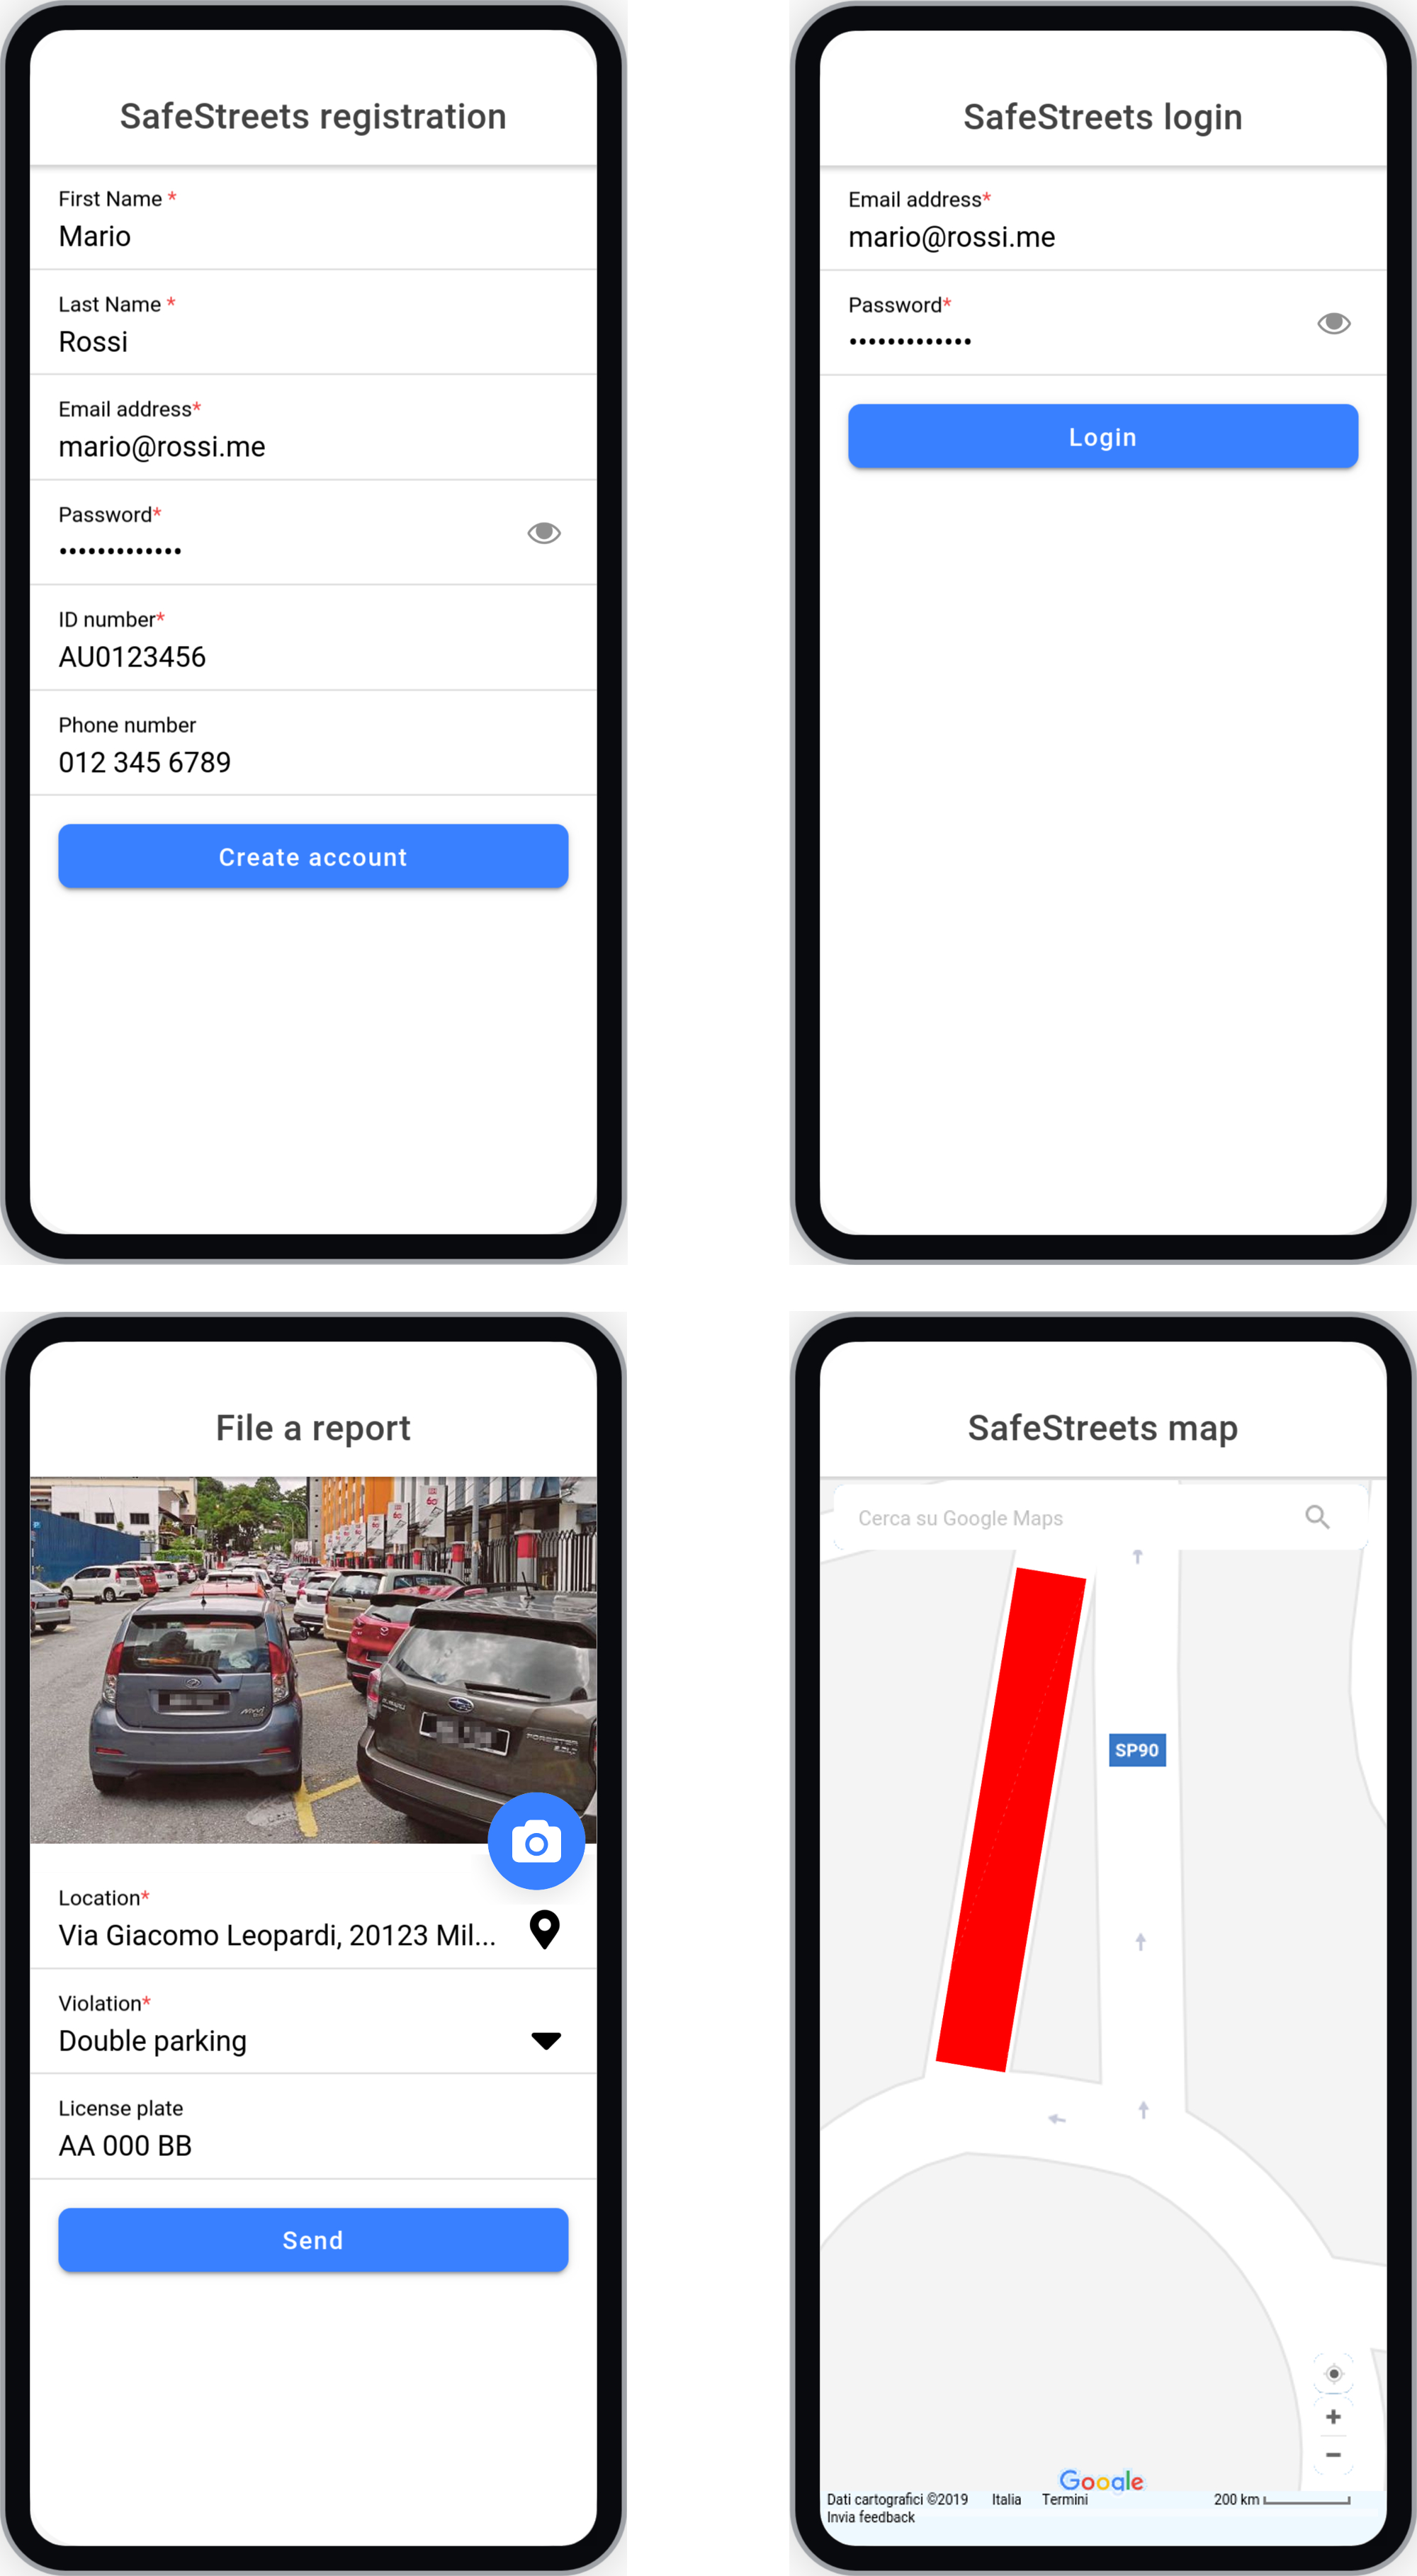
\includegraphics[width=\textwidth,height=.95\textheight,keepaspectratio]{RASD_Images/UserInterface/All.jpg}
  \caption{\textit{UML class diagram}}
\end{figure}
\newpage

\subsection{Hardware Interfaces}
Since the application runs over the Internet, the hardware of both the server and the client needs to be able to connect to the Internet.
\begin{itemize}
  \item Server-side: the hosting platform will provide all the necessary hardware interface.
  \item Client-side: e.g. Wi-Fi, 3G/4G. 
\end{itemize}
Client-side hardware should have a camera in order to have access to all functionalities of the application. It is also recommended, although not mandatory, that client-side hardware is provided with a GPS.


\subsection{Software Interface}
An API provided by SafeStreets allows third parties to access the read-only functionalities offered by the system. This way, third party companies and applications can have access and possibly embed in their software statistical data about accidents and street safety collected by SafeStreets. 
On the other hand, functionalities that involve the creation of new data are meant to be used only within SafeStreets official platforms and are not exposed to third parties.

\subsection{Communication Interface}
SafeStreets will communicate with third parties and with the client application using the standard HTTPS protocol, which guarantees encryption by default.